\section{Simulation Analysis}
\label{sec:simulation}

We simulated the circuit using frequency analysis, using the supplied model of the OP-AMP:

\begin{table}[H]
\addtolength{\tabcolsep}{-4pt}
\caption{Values of capacitances and resistances for various circuit components}
\vspace{-3mm}
\begin{tabular}{|c|c|c|}
\hline
Vcc & $10.0 V$\\
Vee & $10.0 V$\\
C1 & $220 nF$\\
C2 & $220 nF$\\
R1 & $1000 \Omega$\\
R2 & $500 \Omega$\\
R3 & $100 kOhm$\\
R4 & $1000 \Omega$\\
\hline
\end{tabular}
\label{tab:Components}
\end{table}

\par

We simulate the circuit using frequency analysis and max(vin(t))=1, obtaining the following gain in $v_{fin}$, which is the gain at the end of the circuit:

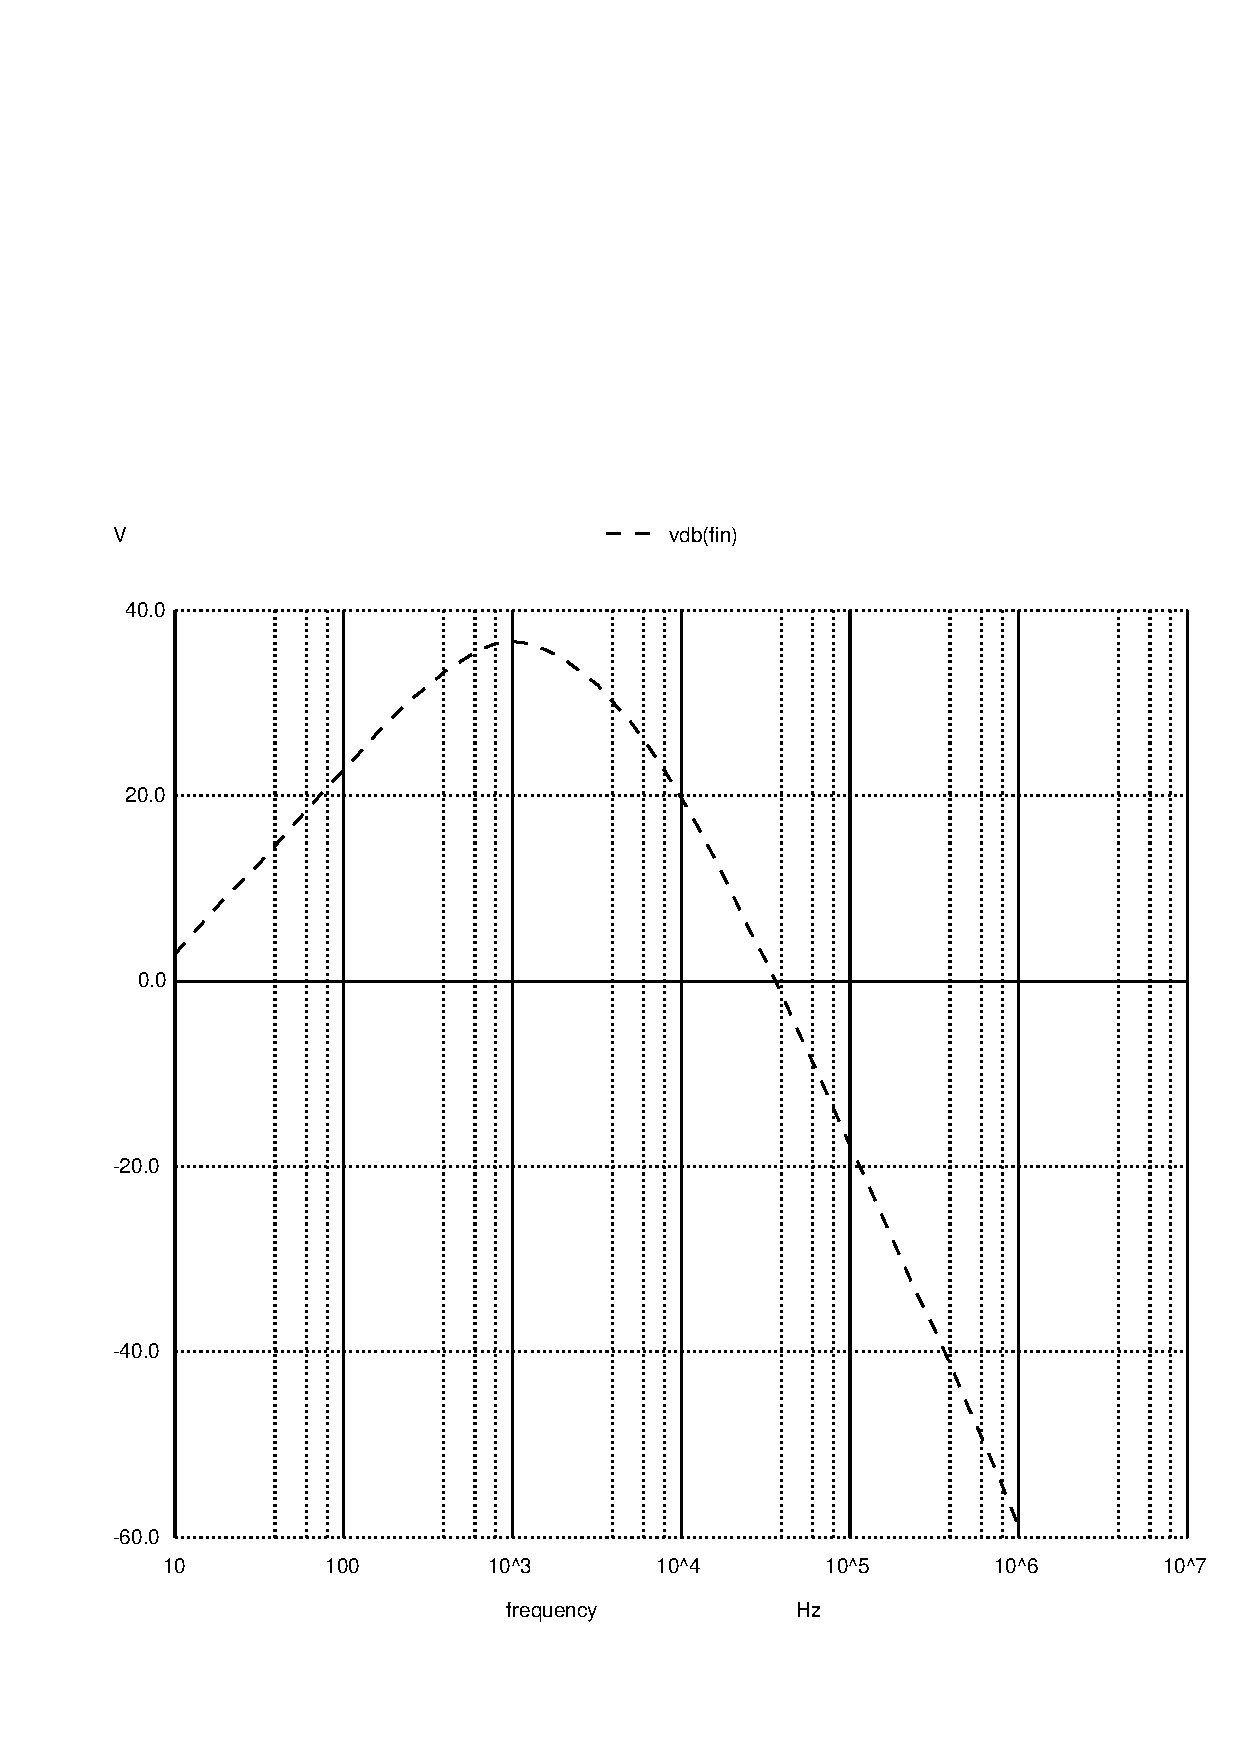
\includegraphics[width=0.8\linewidth]{../sim/vo1f.pdf}

\par

The calculated input impedance is $(990.01+i\cdot 7.32) \Omega$.
A different setup was used to calculate the output impedance which yielded $(-0.09519+i\cdot 7.234) \Omega$.

This circuit has a cost of $113.44$, a maximum gain of $36.55 dB$, central frequency of $1006.5 Hz$.
The calculated merit is therefore $3.9375\cdot 10^{-4}$.
